\chapter{Halbautomatische Erkennung zylindrischer Strukturen}
\label{cha:psoDomes}
	
\dictum[deutsches Sprichwort]{Ein Bild sagt mehr als 1000 Worte.}		
% -------------------------------------------------------------------------------------------------
% -------------------------------------------------------------------------------------------------
% -------------------------------------------------------------------------------------------------
\section{Motivation}

In diesem Kapitel soll das im Rahmen der Masterarbeit entwickelte Verfahren zur halbautomatischen Erfassung 
von zylindrischen Strukturen beschrieben werden. Ziel dieses Verfahrens ist es, die Aufw\"ande f\"ur das Ausmessen von Domstrukturen auf Spritzgu{\ss}teilen ma{\ss}geblich zu verringern (siehe Abschnitt \ref{problem}). 

Ein Dom ist, wie oben im Abschnitt \ref{dome} erl\"autert wurde, ein zylindrischer Vorsprung an einem Bauteil, der h\"aufig ein Befestigungselement aufnimmt. Da solche Dome die Fertigungskosten eines Spritzgu{\ss}teils erheblich steigern, ist es zur Absch\"atzung dieser Kosten notwendig, sowohl die Gesamtanzahl, als auch den Radius und die H\"ohe der einzelnen Zylinderstrukturen zu erfassen.

Das h\"andische Messverfahren, das im Abschnitt \ref{domeMeasure} beschrieben wurde, erlaubt das Messen der Domparameter durch das Platzieren eines parametrischen Zylinders auf einer Domstruktur und des Definierens der Zylinderh\"ohe und des Radius durch grafische Manipulatoren. 
Der parametrische K\"orper wird also durch die H\"ohe, den Radius und die sechs Freiheitsgrade seiner Starrk\"orpertransformation\footnote{Starrkörper besitzen sechs Freiheitsgrade: Sie können in drei Raumrichtungen
verschoben und um die drei Weltkoordinatensystemachsen rotiert werden.} eindeutig beschrieben. Eine zul\"assige Betrachtungsweise der Erfassung einer Domstruktur ist somit die Bestimmung von sinnvollen Werten für diese acht Parameter. Um das Messverfahren zu beschleunigen wurde ein Werkzeug entwickelt, das einerseits die Verschiebungs- und
Rotationswerte durch Analyse der Geometrie in der Umgebung einer Benutzereingabe und anderseits H\"ohe und Radius 
über heuristische Optimierung ermittelt.

\section{Ermittlung der Position und Ausrichtung einer Domstruktur}

Der relativ aufwendige Prozess des h\"andischen Ausmessens einer Domstruktur, der in Abschnitt \ref{domeMeasure} beschrieben wurde, kann zun\"achst beschleunigt werden, indem der Benutzer anstatt eine Punktwolke zu definieren, nur ein Dreieck der Oberfläche selektiert. Ausgehend von diesem Dreieck wird dann ein sogenannter Region Growing Prozess gestartet, der sukzessive benachbarte Dreiecke, die eine bestimmte Eigenschaft besitzen, einer Suchmenge hinzuf\"ugt.
Algorithmus \ref{alg:regionGrowing} beschreibt diese Vorgehensweise im allgemeinen.

\begin{algorithm}[H]
 \SetLine % For v3.9
 %\SetAlgoLined % For previous releases [?]
 \KwData{Dreieck $D_{S}$}
 \KwResult{$R$: Menge an Dreiecken mit einer bestimmten Eigenschaft}
 Erzeuge Stack $S$\;
 Füge $D_{S}$ zu $S$ hinzu\;
 \While{$S$ ist nicht leer}{
  Nehme oberstes Element $D$ vom Stack $S$\;
  Erzeuge Liste $N_{D}$ der Nachbarn von $D$\;
  \For{alle Dreiecke $D_{i}$ aus $N_{D}$}{
  \If{$D_{i}$ erf\"ullt die Zieleigenschaft und $D_{i}$ ist nicht in $R$ enthalten}{
     Lege $D_{i}$ auf $S$\;
   }
  }
  Erzeuge Liste $N_{D}$ der Nachbarn von $D$\;
  Füge $D$ zu $R$ hinzu\;
 }
 \caption{Region Growing}
 \label{alg:regionGrowing}
\end{algorithm}

Die gesuchte Eigenschaft ist hier eine \"ahnlich ausgerichtete Dreiecksnormale. Auf diese Weise kann, wenn der Benutzer ein Dreieck der planaren Zylinderoberseite selektiert, mit einem Klick die ganze Kappe ausgew\"ahlt werden.
Als Position des zu platzierenden Zylinders wird der Schwerpunkt der Zylinderkappe genutzt, der sich folgenderma{\ss}en berechnen l\"a{\ss}t:

\begin{equation}
v=\frac{\sum_{i}  a(v_{i})v_{i}}{\sum_{i}  a(v_{i})}
\end{equation}

Hier ist $v_{i}$ der Dreiecksmittelpunkt und  $a(v_{i})$ die Fläche des Dreiecks. Anschlie{\ss}end können die Scheitelpunkte der Dreiecke als Punktwolke interpretiert werden, f\"ur die mit Hilfe der Hauptkomponentenanalyse eine Best-Fitting Plane erzeugt werden, deren Normale die Rotation des Zylinders definiert. 

\subsection{Bestimmung der Best-Fitting Plane}
\label{subsec:pca}

Eine \textit{Best-Fitting Plane} ist diejenige Ebene, die den aufsummierten orthogonalen Abstand der Punkte zur Ebene minimiert (siehe Abbildung \ref{im:pca}).

 Sie wird aus einer Menge an Dreiecken mit der klassischen Methode, die auf der Hauptkomponentenanalyse (eng \textit{Principal Components Analysis}, kurz PCA) basiert. Genauer wird folgenderma{\ss}en eine Kovarianzmatrix  ${Cov}_{v}$ aus den Vertices der Dreiecke erzeugt:

\begin{equation}
{Cov_{v} =  \sum_{i} a(v_{i})(v_{i}-v)(v_{i}-v)^{T}}
\end{equation}

Die Best-Fitting Plane verläuft durch den Schwerpunkt $a(v)$, ihre Normale $n$ ist der mit dem kleinsten Eigenwert korrespondierende Eigenvektor von ${Cov}_{v}$.

\begin{figure}[ht]
\centering
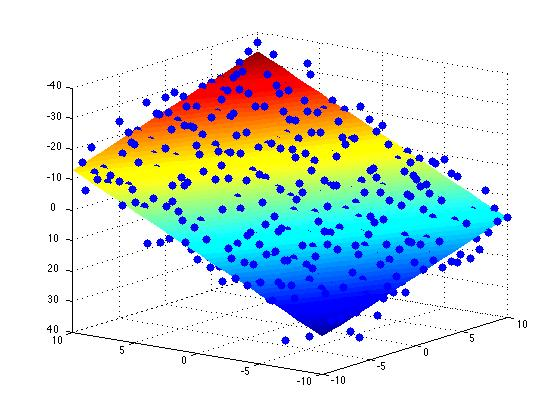
\includegraphics[width=10cm]{graphics/planefit.jpg}
\caption{Best Fitting Plane für eine dreidimensionale Punktwolke.}
\label{im:pca}
\end{figure}

\section{Heuristische Optimierung}
\label{opti}

Ein Optimierungsproblem im mathematischen Sinn ist die Aufgabe, für eine Funktion eine Menge aus Eingabewerten zu finden, so das der Funktion einen minimalen Wert annimmt, wobei in der Regel eine Beschr\"ankung der Eingabewerte vorliegt. Die beste Vorgehensweise hierf\"ur h\"angt von der Art der Bewertungsfunktion ab. Ist diese linear, lassen sich solche Probleme mit Hilfe von Verfahren, die auf dem  Simplex-Algorithmus basieren, effizient l\"osen.

Handelt es sich nicht um lineare Zielfunktionen, sind analytische L\"osungsverfahren meistens sehr ineffizient und das systematische Durchsuchen des L\"oesungsraums ist aufgrund der Problemgr\"o{\ss}e nicht m\"oglich. F\"ur solche Probleme werden in der Informatik oft heuristische Optimierungsverfahren eingesetzt. Diese Verfahren generieren L\"osungen anhand einer definierten Vorgehensweise und verbessern diese suzessive, bis ein Abbruchkriterium, beispielsweise die Anzahl der Iterationen, erreicht ist. Im Folgenden werden drei heuristische Optimierungsverfahren kurz erl\"autert: Simulated Annealing, Evolution\"are Algorithmen und Partikelschwarmoptimierung. 

\textbf{\textit{Simulated Annealing}} (SA, siehe \cite{Kirkpatrik}) imitiert das Abkühlverhalten von Metallen. Kühlen diese langsam ab, haben die Atome ausreichend Zeit, sich zu ordnen und eine stabile Kristallstruktur zu bilden. Der Algorithmus betrachtet einen Punkt im n-dimensionalen L\"osungsraum, der schrittweise in Richtung eines Optimums bewegt wird. Vor jeder Bewegung wird die Zielposition bewertet: Fällt die Bewertung besser aus, als die aktuelle Position, wird die Bewegung durchgeführt. Fällt sie schlechter aus, wird sie nur mit einer gewissen Wahrscheinlichkeit durchgef\"uhrt, die mit jedem Schritt sukzessive verringert wird.Diese Wahrscheinlichkeit entspricht der Temperatur des metallurgischen Abkühlungsprozesses und dient dazu, lokale Minima zu \"uberwinden.

\begin{figure}[ht]
\centering
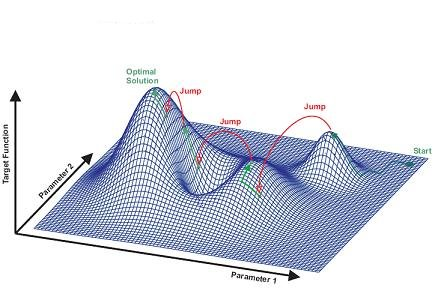
\includegraphics[width=10cm]{graphics/SimAnn.jpg}
\caption{Simulated Annealing in einem zweidimensionalen L\"osungsraum}
\label{fig6}
\end{figure}

\textbf{\textit{Evolution\"are Algorithmen} (EA)} sind eine Familie von Optimierungsverfahren, die sich das Prinzip der Selektion des Bestangepassten ("`\textit{Survival of the fittest}"') der nat\"urlichen Evolution zum Vorbild nehmen. Hierbei wird ein Punkt im L\"osungsraum als Individuum und eine Menge von Punkten als Population bezeichnet. Zu Beginn des Optimierungsverfahren wird der 
L\"osungsraum mit einer randomisierten Population "`bev\"olkert"', die zun\"achst mit einer Zielfunktion (in diesem Zusammenhang oft Fitness-Funktion) bewertet werden. Die am schlechtesten bewerteten Individuen werden verworfen, w\"arend aus den Verbliebenen die n\"achste Population durch Anwendung von sogenannten "`Evolutionären Operatoren"' erzeugt wird, beispielsweise Mutation
(leichtes Verändern eines Individuums) und Rekombination (Mischen der Gene zweier Individuen, oft auch als Crossover bezeichnet).
Dieser Zyklus aus Selektion, Crossover und Mutation wird solange wiederholt, bis ein vorgegebenes Abbruchkriterium (z. B. Anzahl der Generationen) erreicht ist.
Es werden die Hauptforschungsrichtungen Evolution\"are Programmierung (\cite{FogelAIsimEvo}), Genetische Algorithmen (\cite{GoldbergAISimEvo}) und Genetische Programmierung (\cite{KozaAIsimEvo}) unterschieden, die sich bez\"uglich der Datenstrukturen, Selektionsmethoden und der Operatoren unterscheiden.

Als \textbf{\textit{Partikelschwarmoptimierung} (PSO)} wird ein Optimierungsverfahren bezeichnet, das nach dem Vorbild nat\"urlichen Schwarmverhaltens von beispielsweise Fischen oder V\"ogeln eine L\"osung f\"ur das Optimierungsproblem sucht. Die hier beschriebene Version der PSO wurde zuerst 1995 in einer Forschungsarbeit von J. Kennedy and R. Eberhart präsentiert \cite{kennedyPSOConfPaper}. \"Ahnlich den evolution\"aren Algorithmen wird bei der Partikelschwarmoptimierung initial eine zuf\"allige  Menge vom Punkten im L\"osungsraum, die hier als Partikel bezeichnet werden, erzeugt. Der Partikelschwarm wird nun schrittweise durch den L\"osungsraum bewegt, wobei benachbarte Partikel vor jedem Schritt die beste Position, die ein Partikel bisher gefunden hat, austauschen k\"onnen. Welche Partikel miteinander kommunizieren k\"onnen wird durch die sogenannte Nachbarschaftstopologie bestimmt. 
Ein Partikel h\"alt somit zus\"atzlich zur Position $\vv{x}$ noch eine Bewegungsrichtung $\vv{v}$, die bisher beste gefundene Position als $\vv{p}_{best}$ und die beste Position seiner Umgebung als $\vv{n}_{best}$. Nach jedem Zeitschritt wird die Position und die Bewegungsrichtung (der Vektor $\vv{v}$ ist nicht normalisiert, er beinhaltet die Geschwindigkeit und Richtung) eines Partikels anhand folgender Formeln angepasst:

\begin{equation}
\vv{v}_{i,t+1} = \omega\cdot\vv{v}_{i,t}+c_{1}\cdot\vv{U}_{1}[0,1]\bigotimes(\vv{p}_{best,i,t})-\vv{x}_{i,t})
+c_{2}\cdot\vv{U}_{2}[0,1]\bigotimes(\vv{g}_{best,i,t})-\vv{x}_{i,t})
\end{equation}

\begin{equation}
\vv{x}_{i,t+1} = \vv{x}_{i,t} + \vv{v}_{i,t+1}
\end{equation}

Hierbei ist $t$ der Interationsz\"ahler, $\vv{U}_{k}[0,1]$ Zufallsvektoren und die Parameter $\omega$, $c_{1}$, $c_{1}$ bestimmen den Einflu{\ss}  der Position des vorigen Zeitschritts und der kognitiven und sozialen Komponenten.

%Hier Beschreibung des Problems,,,seperabel warum? multimadal? 
\section{Zielfunktion des Optimierungsproblems}



\subsection{Kollisionsvermeidung}

\subsection{Aufsummierter quadratischer Abstand (SSD)}

\section{Implementierung und Ergebnisse}

